% To create rdesigneur slide
\documentclass[crop,tikz]{standalone}
\begin{document}


% From here 
% http://tex.stackexchange.com/questions/183848/how-draw-part-of-ring-or-broken-ring-in-tikz
% \drawsector[draw options]{text radius}{width}{start angle}{delta angle}{text}
\newcommand{\drawsector}[6][]{
    \draw[#1,opacity=0.5] (#4:{#2-.5*#3}) arc [start angle = #4, delta angle=-#5, radius={#2-.5*#3}]--++({#4-#5}:#3) arc [start angle = {#4- #5}, delta angle=#5, radius={#2+.5*#3}] --cycle;
    \draw[decorate,decoration={raise=-3pt, text along path, text=#6, text align={align=center}}] (#4:#2) arc(#4:(#4-#5):#2);
}

\usetikzlibrary{scopes, decorations.text}

\begin{tikzpicture}[scale=1,
    , every node/.style={ circle }
    ]
    \node (rdesigneur) at (0,0) {};

    { [ xshift=-0.5\textwidth,yshift=0.3\textwidth]
        % neuromorpho 
        \node[rectangle] (neuromorphoSummary) {
            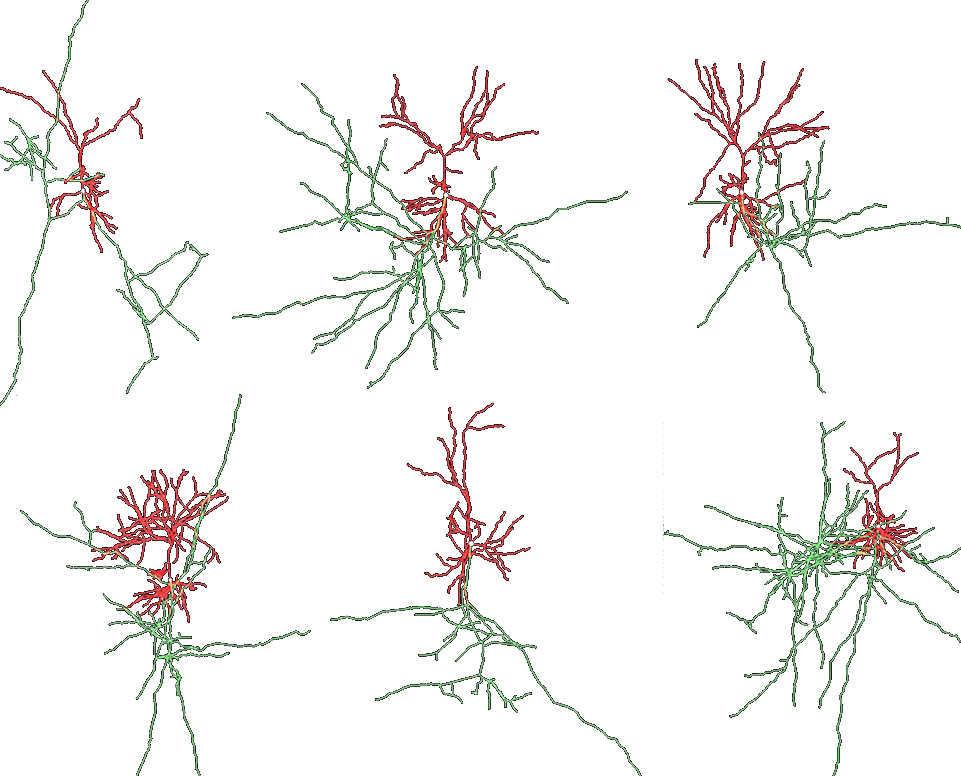
\includegraphics[angle=90,width=0.5\textwidth]{./../_images/neuromorpho_summary.png}
        };
    }

    { [ yshift=0.5\textwidth ]
        \node[circle] (channelExample)  {
            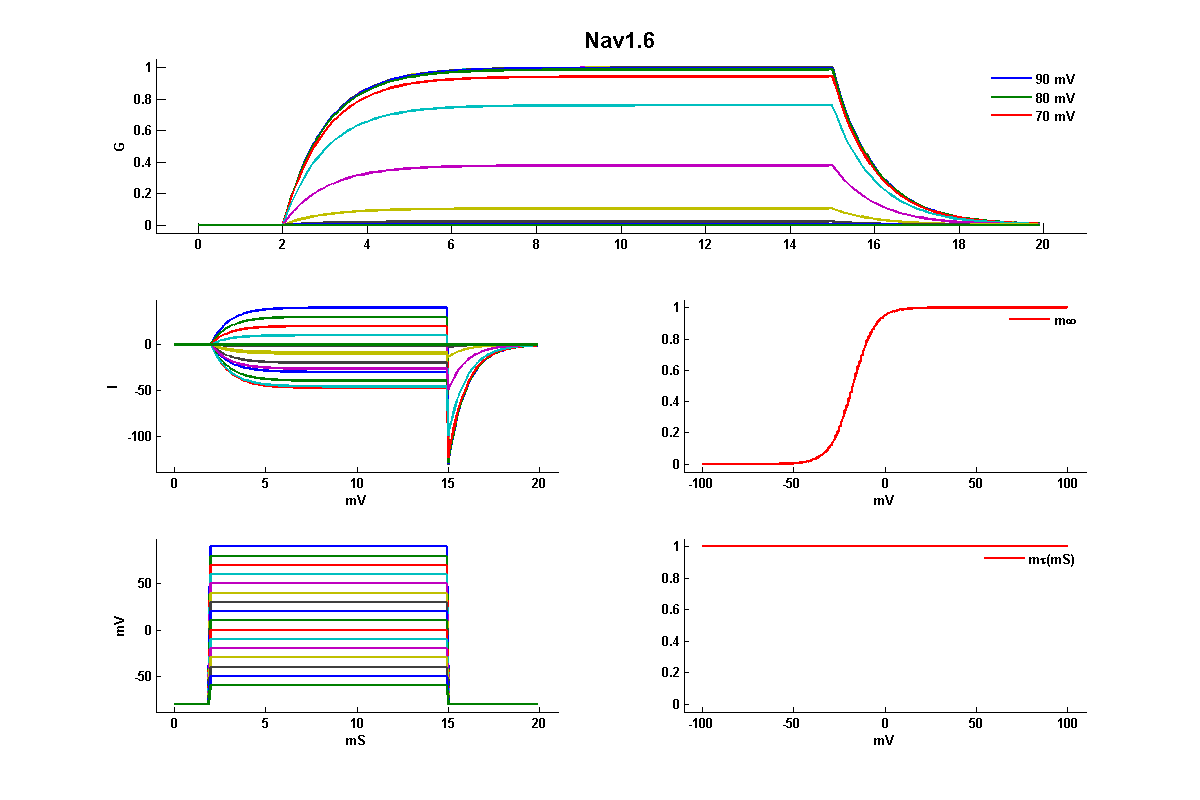
\includegraphics[width=0.4\textwidth]{./../_images/channelpedia_example.png}
        };
    }

    { [ yshift=0.1\textwidth, xshift=0.5\textwidth ] 

        \node[] (doqcs) { 
            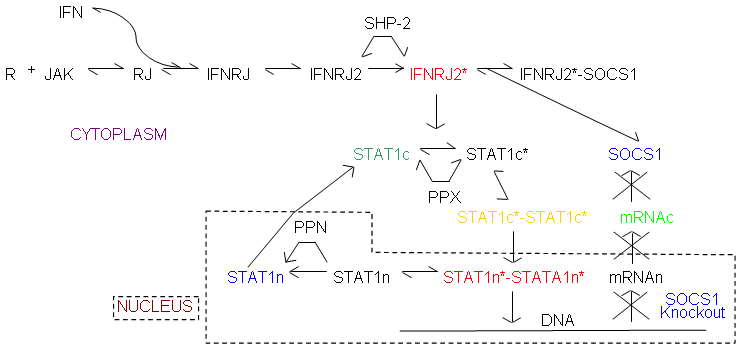
\includegraphics[width=0.5\textwidth]{./../_images/acc67.png}
        };

        \node[] (doqcs2)  at (doqcs.north) {
            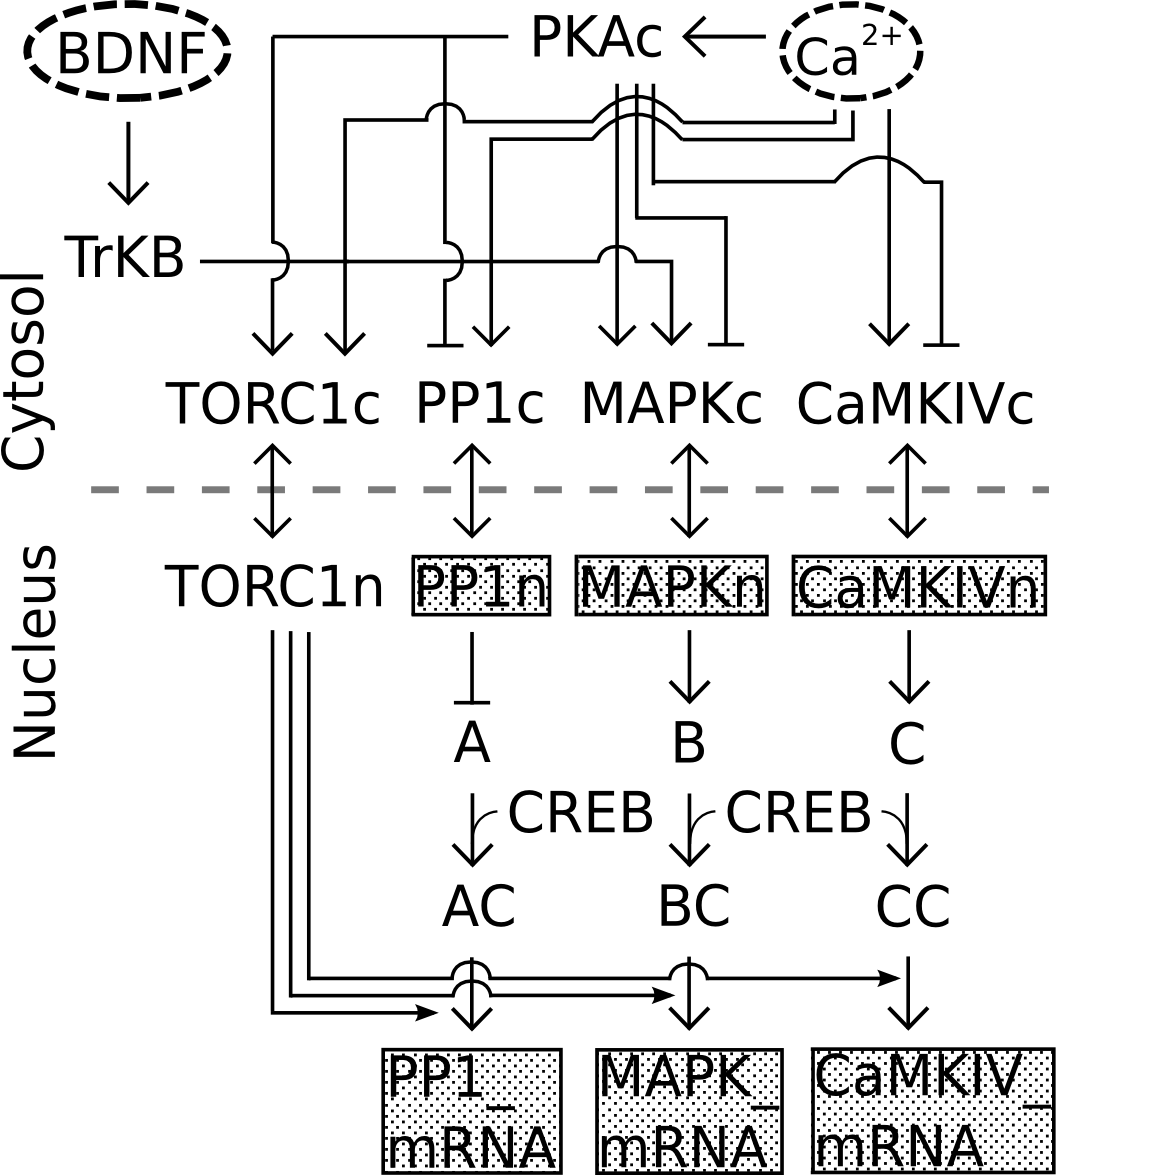
\includegraphics[width=0.4\textwidth]{../_images/acc95.png}
        };
    }

    \node [circle, draw, minimum size=7cm, fill=blue!10] (rdesigneur) at (0,0) {\texttt{moose.redesigneur}};

    { [ draw=none,fill=red!10 ]
        \drawsector[fill=blue,opacity=0.3]{4}{1}{210}{80}{Electrical Models};
        \drawsector[draw=none,fill=red!10]{4.75}{0.5}{170}{40}{OpenSourceBrain};
        \drawsector[draw=none,fill=red!10]{4.75}{0.5}{210}{30}{NeuroMorpho};


        \drawsector[fill=yellow, opacity=0.3]{4}{1}{120}{40}{Channels};
        \drawsector[draw=none,fill=red!10]{4.75}{0.5}{120}{30}{Channelpedia};

        \drawsector[fill=yellow, opacity=0.3]{3}{0.5}{150}{70}{Channel
            Distribution};

        \drawsector[fill=red, opacity=0.3]{4}{1}{70}{80}{Chemical Models};
        \drawsector[draw=none,fill=red!10]{4.75}{0.5}{70}{20}{SBML};
        \drawsector[draw=none,fill=red!10]{4.75}{0.5}{50}{20}{DOQCS};
        \drawsector[draw=none,fill=red!10]{4.75}{0.5}{30}{30}{Bio Models};

    }



\end{tikzpicture}    


\end{document}

